\begin{questions}
\question{
Sinc(x) definition of the delta function
}
\begin{solution}

First we will calculate the given integral

\begin{equation}
  \begin{aligned}[b]
    \frac{1}{2\pi} \int_{-Z}^Z e^{ikx}dk &= \left.\frac{e^{ikx}}{2\pi ix} \right|_{-Z}^Z ,\\
    &= \frac{e^{iZx} - e^{-iZx}}{2\pi ix},\\
    &= \frac{1}{\pi x}\frac{e^{iZx} - e^{-iZx}}{2i},\\
    &= \frac{\sin(Zx)}{\pi x}.
    \label{int:delt}
  \end{aligned}
\end{equation}

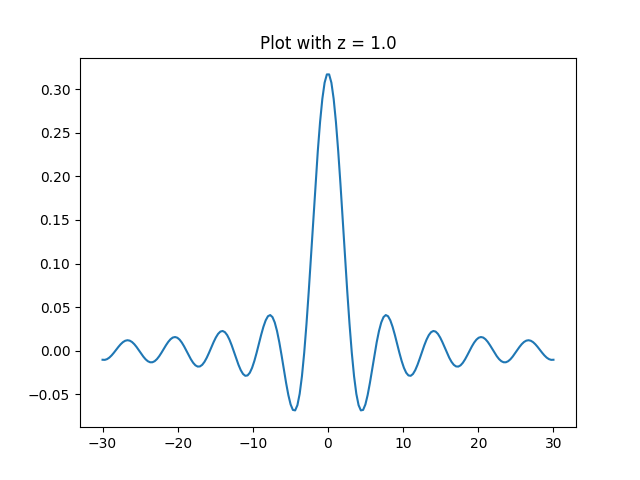
\includegraphics[width=50mm]{delt1.png}
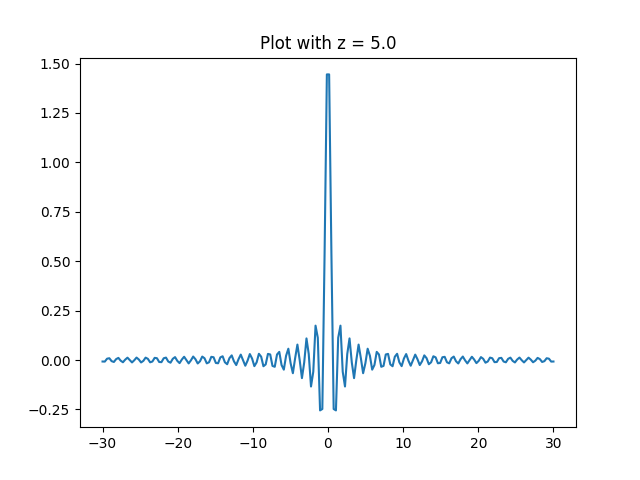
\includegraphics[width=50mm]{delt5.png}
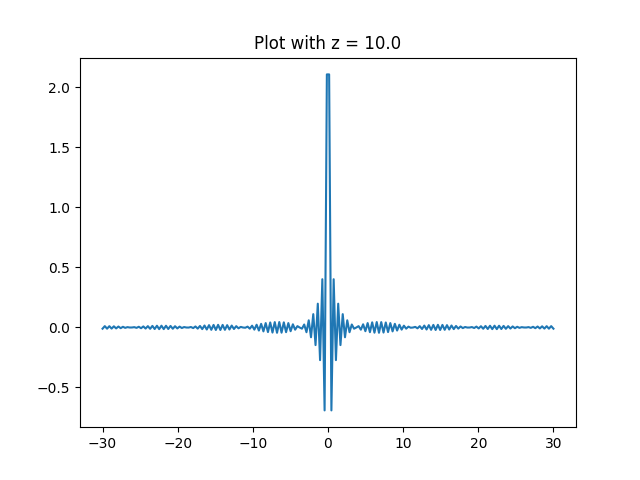
\includegraphics[width=50mm]{delt10.png}\label{del:plots}

\hspace{25mm}a)\hspace{47mm}b)\hspace{48mm}c)

 \captionof{figure}{Plots for eq. \ref{int:delt} using a) $Z=1$, b) $Z=5$, and c) $Z=10$}
 \vspace{1cm}

 \textbf{Where does it have its maximum value?} At x=0.\\

 \textbf{What happens when increasing Z?} The peak rises but also narrows.\\

 \end{solution}

 \question{The integral of $\delta$ is one.}
 \begin{solution}

 Now we need to show that the integral of delta is one

 \begin{equation}
   \begin{aligned}[b]
     \int_{-\infty}^\infty \delta(x) dx &= \int_{-\infty}^\infty \frac{1}{2\pi} \lim_{Z\rightarrow \infty} \int_{-Z}^Z e^{ikx}dk,\\
     &= \int_{-\infty}^\infty \lim_{Z\rightarrow \infty} \frac{\sin(Zx)}{\pi x},\quad  \textnormal{using eq. \ref{int:delt}},\\
     &=\lim_{Z\rightarrow \infty} \int_{-\infty}^\infty  \frac{\sin(Zx)}{\pi x}, \quad \textnormal{linearity},\\
     &= \frac{1}{\pi}\lim_{Z\rightarrow \infty} \int_{-\infty}^\infty \frac{\sin(x')}{ x'}dx', \quad \textnormal{change of variable $x'=Zx$},\\
     &= \frac{1}{\pi}\lim_{Z\rightarrow \infty} \pi,\\
     &= \frac{\pi}{\pi} = 1 \quad _\blacksquare. \label{integral}
   \end{aligned}
 \end{equation}
 Being strict we should have changed the $Z$ on the limit when we changed variable, but as we saw the final result of the integral was not affected by the value of $Z$. So we can omit that step in order to avoid unnecessary calculations.
\end{solution}

\question{Fourier transform of $\delta$}
\begin{solution}
  Let's begin with the definition
  \begin{equation*}
    \begin{aligned}
      \delta(k') &= \int_{-\infty}^\infty e^{-ik'x}\delta(x)dx,\\
      &= \int_{-\infty}^\infty e^{-ik'x}\left(\frac{1}{2\pi}\int_{-\infty}^\infty e^{ikx}dk\right)dx, \quad \textnormal{definition of $\delta(x)$,}\\
      &= \frac{1}{2\pi}\int_{-\infty}^\infty \int_{-\infty}^\infty e^{-ik'x} e^{ikx}dkdx,\\
      &= \frac{1}{2\pi}\int_{-\infty}^\infty \int_{-\infty}^\infty  e^{i(k-k')x}dkdx,\\
      &= \frac{1}{2\pi}\int_{-\infty}^\infty \int_{-\infty}^\infty  e^{ik''x}dk''dx, \quad \textnormal{variable change $k'' = k-k'$},\\
      &= \int_{-\infty}^\infty \left( \frac{1}{2\pi}\int_{-\infty}^\infty  e^{ik''x}dk''\right)dx,\\
      &= \int_{-\infty}^\infty \delta(x) dx, \quad \textnormal{by definition},\\
      &= 1, \quad \textnormal{using eq. \ref{integral}}.
    \end{aligned}
  \end{equation*}

\end{solution}

\question{Properties of Dirac's delta}
\begin{solution}
 Here we show a couple of properties of this distribution
 \begin{eqnarray}
   \int_{-\infty}^\infty f(x)\delta(x)dx = f(0).\\
   \int_{-\infty}^\infty \delta(\alpha x)dx = \frac{1}{|\alpha|}.\\
   \delta(-x) = \delta(x).\\
   \int_{-\infty}^\infty f(t)\delta(t-T)dx = f(T).\\
   \int_{-\infty}^\infty f(x)\delta(x-a) = \int_{-\infty}^\infty f(a)\delta(x-a).\\
   \int_{-\infty}^\infty \delta(a-x)\delta(x-b)dx = \delta(a-b).
 \end{eqnarray}
\end{solution}

\question{Properties of Fourier transforms}
\begin{solution}
We will denote the Fourier transform operation  with a hat. For $a,b\in \mathbb{C}$, if $h(x) = af(x) + bg(x)$ then
\begin{eqnarray}
  \hat{h}(\xi) = a\hat{f}(\xi) +b\hat{g}(\xi).
\end{eqnarray}
For $x_0\in \mathbb{R}$, if $h(x)=f(x-x_0)$, then
\begin{equation}
  \hat{h}(\xi) = e^{-2\pi ix_0\xi}\hat{f}(\xi).
\end{equation}
For $\xi_0\in \mathbb{R}$, if $h(x)=e^{2\pi ix\xi_0}f(x)$, then
\begin{equation}
  \hat{h}(\xi) = \hat{f}(\xi - \xi_0).
\end{equation}
For $a\neq 0 \in \mathbb{R}$ if $h(x) = f(ax)$ then
\begin{equation}
  \hat{h}(\xi) = \frac{1}{|a|}f\left(\frac{\xi}{a}\right).
\end{equation}
If $h(x) = \overline{f(x)}$, then
\begin{equation}
  \hat{h}(\xi) = \overline{\hat{f}(-\xi)}.
\end{equation}
But we have to be careful with those $2\pi$ factors because they depend on the definition of the Fourier transform, and the inverse Fourier transform.
\end{solution}

\end{questions}

% \includegraphics[width=75mm]{}\label{}
%
%
%  \captionof{figure}{}
